\documentclass[a4paper,11pt]{article}
\usepackage[portuguese]{babel}
\usepackage{graphicx}
\usepackage{amsmath}
\usepackage{minted}
\usepackage{mdframed}

\usepackage[twoside,verbose,body={16cm,24cm},
left=25mm,top=20mm]{geometry}


\title{Cálculo de Programas \\ Resolução - Ficha 02}
\author{Eduardo Freitas Fernandes}
\date{2025}

\setminted{
	frame=single,
	tabsize=4,
	breaklines=true
}


\begin{document}
	
\maketitle
	
\noindent \underline{\textbf{Exercício 1}}\\

\begin{minipage}{0.45\textwidth}
\begin{mdframed}
	\[
	\begin{aligned}
		\pi_1 \cdot (f \times g) \  (x, y) 
		= \  &\{\text{def. composição}\}\\
		&\pi_1 ((f \times g) (x, y)) \\
		= \  &\{\text{(F1)}\}\\
		&\pi_1 (f \  x, g \  y) \\
		= \  &\{\text{(F2)}\}\\
		&f \  x \\
		= \  &\{\text{(F2)}\}\\
		&f (\pi_1 (x, y)) \\
		= \  &\{\text{def. composição}\}\\
		&f \cdot \pi_1
	\end{aligned}
	\]
\end{mdframed}	
\end{minipage}
\hfill
\begin{minipage}{0.45\textwidth}
\begin{mdframed}
	\[
	\begin{aligned}
		\pi_2 \cdot (f \times g) \  (x, y) 
		= \  &\{\text{def. composição}\}\\
		&\pi_2 ((f \times g) (x, y)) \\
		= \  &\{\text{(F1)}\}\\
		&\pi_2 (f \  x, g \  y) \\
		= \  &\{\text{(F2)}\}\\
		&g \  y \\
		= \  &\{\text{(F2)}\}\\
		&g (\pi_2 (x, y)) \\
		= \  &\{\text{def. composição}\}\\
		&g \cdot \pi_2
	\end{aligned}
	\]
\end{mdframed}
\end{minipage}

\begin{center}
\begin{minipage}{0.5\textwidth}
	\begin{mdframed}
		\[
		\begin{aligned}
			(f \times g) \  (x, y)
			= \  &\{\text{(F1)}\}\\
			&(f \  x, g \  y) \\
			= \  &\{\text{(F2)}\}\\
			&(f (\pi_1 (x, y)), g (\pi_2 (x, y))) \\
			= \  &\{\text{def. composição}\}\\
			&(f \cdot \pi_1, g \cdot \pi_2) \\
			= \  &\{\text{def. split}\}\\
			&\langle f \cdot \pi_1, g \cdot \pi_2 \rangle \\
		\end{aligned}
		\]
	\end{mdframed}
\end{minipage}
\end{center}

\newpage

	\noindent \underline{\textbf{Exercício 2}}
	
\begin{center}
	\begin{minipage}{0.65\textwidth}
		\begin{mdframed}
			\[
			\begin{aligned}
				xor \cdot (and \times id) \  ((a, b), c)
				= \  &\{\text{def. composição}\}\\
				&xor ((and \times id) \  ((a, b), c))\\
				= \  &\{\text{(F1)}\}\\
				&xor(and (a, b), \ id \  c)\\
				= \  &\{\text{def. and, def. id}\}\\
				&xor(a \land b, c)\\
				= \  &\{\text{def. xor}\}\\
				&(a \land b) \oplus c
			\end{aligned}
			\]
		\end{mdframed}
	\end{minipage}
\end{center}
	
	
	\noindent \underline{\textbf{Exercício 3}}
	
	\begin{verbatim}
		ghci> :l Cp.hs
		ghci> xor (x,y) = x /= y
		ghci> and (x,y) = x && y
		ghci> f = xor . (and >< id)
		ghci> f ((True, True), False)
		True
		ghci> f ((True, True), True)
		False
		ghci> f ((False, True), True)
		True
		ghci> f ((True, False), True)
		True
	\end{verbatim}
	
	
	\noindent \underline{\textbf{Exercício 4}}
	\[
		id = \langle f, g \rangle \iff
		\begin{cases}
			\pi_1 \cdot id = f\\
			\pi_2 \cdot id = g\\
		\end{cases}
		\iff
		\begin{cases}
			\pi_1 = f \\
			\pi_2 = g \\
		\end{cases}
		\iff id = \langle \pi_1, \pi_2 \rangle
	\]
	
	\noindent Seja $ k = id $, ao aplicar a propriedade \textit{universal-$\times$} obtemos a propriedade \textit{reflexão-$\times$}.\\
	
	
	\noindent \underline{\textbf{Exercício 5}}
	\begin{center}
		\begin{minipage}{0.45\textwidth}
			\begin{mdframed}
				\[
				\begin{aligned}
					&\underbrace{\langle h, k\rangle \cdot f}_{k} = \underbrace{\langle h \cdot f, k \cdot f \rangle}_{\langle h, f \rangle} \\
					\iff &\{\text{(F7)}\} \\
					&\begin{cases}
						\pi_1 \cdot \langle h, k \rangle \cdot f = h \cdot f \\
						\pi_2 \cdot \langle h, k \rangle \cdot f = k \cdot f \\
					\end{cases}\\
					\iff &\{\text{Cancelamento-$\times$}\} \\
					&\begin{cases}
						h \cdot f = h \cdot f \\
						k \cdot f = k \cdot f\\
					\end{cases}
				\end{aligned}
				\]
			\end{mdframed}
		\end{minipage}
	\end{center}
	
	
	\noindent \underline{\textbf{Exercício 6}}
	\begin{center}
		\begin{minipage}{0.45\textwidth}
			\begin{mdframed}
				\[
				\begin{aligned}
					dup \cdot f \  x
					= \  &\{\text{natural-id}\} \\
					&dup \cdot f \cdot id \  x \\
					= \  &\{\text{def. composição}\} \\
					&dup(f(id \  x)) \\
					= \  &\{\text{def. dup}\} \\
					&( f(id \  x), f(id \  x) ) \\
					= \  &\{\text{def. composição}\} \\
					&\langle f \cdot id, f \cdot id \rangle \\
					= \  &\{\text{fusão-x}\} \\
					&\langle f , f \rangle \cdot id \\
					= \  &\{\text{natural-id}\} \\
					&\langle f , f \rangle
				\end{aligned}
				\]
			\end{mdframed}
		\end{minipage}
	\end{center}
	
	
	\noindent \underline{\textbf{Exercício 7}}
	\begin{center}
		\begin{minipage}{0.4\textwidth}
			\begin{mdframed}
				\[
				\begin{aligned}
					&\underbrace{\underline{(b, a)}}_{k} = \underbrace{\langle \underline{b}, \underline{a} \rangle}_{\langle f, g \rangle} \\
					\iff &\{\text{universal-$\times$}\} \\
					&\begin{cases}
						\pi_1 \cdot \underline{(b, a)} = \underline{b} \\
						\pi_2 \cdot \underline{(b, a)} = \underline{a} \\
					\end{cases}\\
					\iff &\{\text{absorção-const}\} \\
					&\begin{cases}
						\underline{\pi_1 (b, a)} = \underline{b} \\
						\underline{\pi_2 (b, a)} = \underline{a} \\
					\end{cases}\\
					\iff &\{\text{cancelamento-$\times$}\} \\
					&\begin{cases}
						\underline{b} = \underline{b} \\
						\underline{a} = \underline{a} \\
					\end{cases}
				\end{aligned}
				\]
			\end{mdframed}
		\end{minipage}
	\end{center}
	
	
	\noindent \underline{\textbf{Exercício 8}}
	\\
	
	\begin{minipage}{0.47\textwidth}
		\begin{mdframed}
			\[
			\begin{aligned}
				&(g \times f) \cdot swap \\
				= \  &\{\text{def-$\times$}\}\\
				&\langle g \cdot \pi_1, f \cdot \pi_2 \rangle \cdot swap \\
				= \  &\{\text{fusão-$\times$}\}\\
				&\langle g \cdot \pi_1 \cdot swap, f \cdot \pi_2 \cdot swap \rangle \\
				= \  &\{\text{def. swap}\}\\
				&\langle g \cdot \pi_1 \cdot \langle \pi_2, \pi_1 \rangle, f \cdot \pi_2 \cdot \langle \pi_2, \pi_1 \rangle \rangle \\
				= \  &\{\text{cancelamento-$\times$}\}\\
				&\langle g \cdot \pi_2 , f \cdot \pi_1 \rangle
			\end{aligned}
			\]
		\end{mdframed}
	\end{minipage}
	\hfill
	\begin{minipage}{0.47\textwidth}
		\begin{mdframed}
			\[
			\begin{aligned}
				&swap \cdot (f \times g) \\
				= \  &\{\text{def. swap}\}\\
				&\langle \pi_2, \pi_1 \rangle \cdot (f \times g)\\
				= \  &\{\text{fusão-$\times$}\}\\
				&\langle \pi_2 \cdot (f \times g), \pi_1 \cdot (f \times g) \rangle \\
				= \  &\{\text{def-$\times$}\}\\
				&\langle \pi_2 \cdot  \langle f \cdot \pi_1, g \cdot \pi_2 \rangle, \pi_1 \cdot  \langle f \cdot \pi_1, g \cdot \pi_2 \rangle \rangle \\
				= \  &\{\text{cancelamento-$\times$}\}\\
				&\langle g \cdot \pi_2 , f \cdot \pi_1 \rangle
			\end{aligned}
			\]
		\end{mdframed}
	\end{minipage}
	
	
	\newpage

	\noindent \underline{\textbf{Exercício 9}}
	
\begin{minted}{haskell}
acronym :: String -> String
acronym = map head . words

short :: String -> String
short = uncurry (++) . (id >< (' ':)) . split head last . words
\end{minted}

\begin{figure}[H]
	\centering
	\fbox{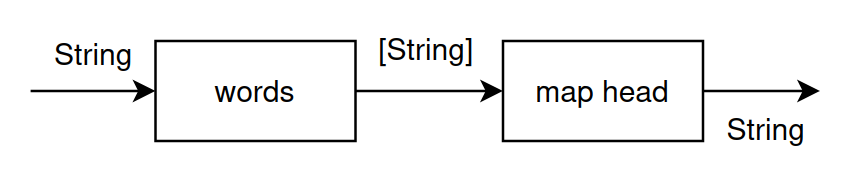
\includegraphics[width=0.5\textwidth]{imgs/acronym.png}}
	\caption{acronym}
\end{figure}
	
\begin{figure}[H]
	\centering
	\fbox{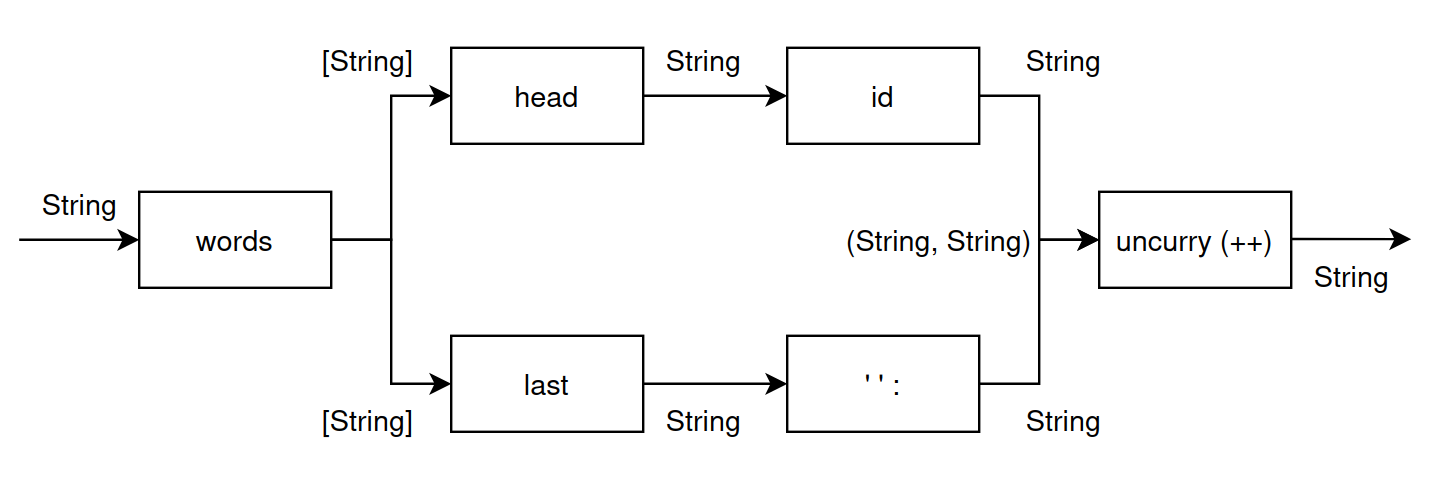
\includegraphics[width=0.75\textwidth]{imgs/short.png}}
	\caption{short}
\end{figure}

	
\end{document}
